% conceitos basicos
% 
% Arrumar este capítulo para conter a descrição de como se calcula os
% limitantes para cada operação
%
Neste capítulo faremos uma apresentação dos conceitos básicos
necessários para o entendimento e desenvolvimento deste trabalho. Na
seção \ref{sec:defin} mostraremos as definições usadas no decorrer
deste trabalho. As seções \ref{sec:rev}, \ref{sec:trans}
e \ref{sec:rev_trans} descrevem, respectivamente, os problemas de
ordenação por reversões, ordenação por transposições e ordenação por
reversões e transposições.

\section{Definições}
\label{sec:defin}
Para todos os problemas usamos as seguintes definições.

\textit{Permutação.} 
Para fins computacionais, um genoma é representado por uma $n$-tupla
de genes, e quando não há genes repetidos essa $n$-tupla é chamada de
permutação. Uma permutação é representada como $\pi =
(~\pi_{1}~\pi_{2}~\ldots~\pi_{n}~)$, para $\pi_{i} \in \mathbb{N}$, $0
< \pi_{i} \leq n$ e $i \neq j \leftrightarrow \pi_{i} \neq \pi_{j}$. A
permutação identidade é representada como $\iota =
(~1~2~3~\ldots~n~)$. Para a demonstração dos eventos, usaremos como
base a permutação $\pi = (~4~7~3~6~2~5~1~)$.

\textit{Eventos de rearranjo.}
Os eventos de rearranjo tratados neste trabalho são os eventos de
transposição e reversão quando ocorrem isoladamente e quando ocorrem
de forma conjunta. Os eventos são representados por $\rho$ e são
aplicados a $\pi$ de uma maneira específica.

\section{Ordenação por Reversões}
\label{sec:rev}
Um evento de reversão ocorre quando um bloco do genoma é
invertido. Uma reversão $\rho(i, j)$, para $1 \leq i < j \leq n$,
aplicada ao genoma $\pi = (~\pi_{1}~\pi_{2}~\ldots~\pi_{n}~)$ gera a
permutação $\rho\pi =
(\pi_{1}~\ldots~\pi_{i-1}~\pi_{j}~\pi_{j-1}~\ldots~\pi_{i+1}$
$\pi_{i}~ \pi_{j+1}~\ldots~\pi_{n})$, caso a orientação de $\pi$ não é
conhecida (Figura~\ref{fig:rev_nao_orientada}), e $\rho\pi =
(\pi_{1}~\ldots~\pi_{i-1}~-\pi_{j}~-\pi_{j-1}~\ldots~-\pi_{i+1}$
$-\pi_{i}~ \pi_{j+1}~\ldots~\pi_{n})$, caso a orientação de $\pi$ é
conhecida (Figura~\ref{fig:rev_orientada}). 

\begin{figure}
  \centering
  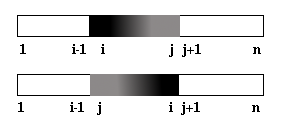
\includegraphics{images/rev_nao_orientada.png} 
  \caption{Reversão em uma permutação não orientada.}
  \label{fig:rev_nao_orientada}
\end{figure}

\begin{figure}
  \centering
  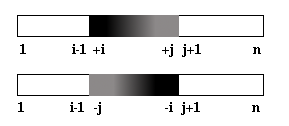
\includegraphics{images/rev_orientada.png}
  \caption{Reversão em uma permutação orientada.}
  \label{fig:rev_orientada}
\end{figure}

A distância de reversão $d_{r}(\pi,\sigma)$ entre duas permutações
$\pi$ e $\sigma$ é o número mínimo $r$ de reversões $\rho_{1}$,
$\rho_{2}$,~$\ldots$~, $\rho_{r}$ tal que
$\pi \rho_{1} \rho_{2}~\ldots~\rho_{r} = \sigma$. Note que a distância
de reversão entre $\pi$ e $\sigma$ é igual à distância de reversão
entre $\sigma^{-1} \pi$ e $\iota$. Então, sem perda de generalidade,
podemos dizer que o problema da distância de reversão é equivalente ao
problema de ordenação por reversões, que é a distância de reversão
entre a permutação $\pi$ e a permutação identidade $\iota$, denotado
por $d_{r}(\pi)$.

Em um estudo inicial sobre este problema, Bafna e
Pevzner~\cite{BafnaPevzner*1996} apresentaram um algoritmo de
aproximação com razão de $1.5$ quando a orientação de genes é
conhecida e $1.75$ caso contrário.

Conhecer a orientação dos genes em um genoma é um fator importante no
problema de reversão, pois existem algoritmos polinomiais para o caso
em que a orientação é conhecida. No caso em que não se conhece a
orientação dos genes o problema de encontrar a distância de reversão
pertence à classe dos problemas NP-Difíceis~\cite{Caprara*1997}.

O primeiro algoritmo polinomial para o problema de reversão com
orientação conhecida foi criado por Hannenhalli e
Pevzner~\cite{HannenhalliPevzner*1995} que fez uso de várias operações
aplicadas a uma estrutura intermediária conhecida como grafo
de \bkp{}. A estratégia usada por Hannenhalli e Pevzner foi
simplificada no trabalho de Bergeron~\cite{Bergeron*2005}. Atualmente
já existe um algoritmo com complexidade
sub quadrática~\cite{TannierSagot*2004} e, quando apenas a distância é
necessária, um algoritmo linear pode ser
usado~\cite{BaderMoretYan*2001}.

Um resultado importante obtido por Meidanis, Walter e
Dias~\cite{MeidanisWalterDias*2000}, mostrou que toda teoria sobre
reversões desenvolvida para genomas lineares pode ser adaptada
facilmente para genomas circulares, que são comuns em seres inferiores
como vírus e bactérias.

Quando a orientação dos genes não é conhecida existem algoritmos de
aproximação que seguiram a ideia do trabalho de Bafna e Pevzner citado
anteriormente como, por exemplo, o algoritmo implementado por Berman,
Hannenhalli e Karpinski~\cite{BermanHannenhalliKarpinski*2002} com
razão de aproximação de $1.375$.

\subsection{Ferramentas para o Problema de Ordenação por Reversões.}
\label{subsec:toolrev}
O conceito de grafo de \bkp{} foi introduzido no trabalho de Bafna e
Pevzner~\cite{BafnaPevzner*1996}. Inicialmente a permutação $\pi$ é
estendida adicionando o elemento $\pi_{0} = 0$ e $\pi_{n+1} =
n+1$. Dois elementos consecutivos $\pi_{i}$ e $\pi_{i+1}$, $0 \le
i \le n$, são \textit{adjacentes} quando $|\pi_{i} - \pi_{i+1}| = 1$,
e são \estr{breakpoints} caso contrário. Define-se um grafo de arestas
coloridas $G(\pi)$ com $n + 2$ vértices \{0, 1,~$\ldots$~, $n$, $n +
1$\}. Unimos os vértices $i$ e $j$ com uma aresta preta se $(i, j)$
for um \estr{breakpoint}. Unimos os vértices $i$ e $j$ com uma aresta
cinza se $|i - j| = 1$ e $i$, $j$ não são consecutivos em
$\pi$. Denotamos por $b_r(\pi)$ o número de \bkp{} existentes em
$\pi$. A Figura~\ref{fig:rev_grafo_bkp} mostra o grafo de \bkp{} da
permutação $\pi = (~4~7~3~6~2~5~1~)$.

\begin{figure}[h]
  \centering 
  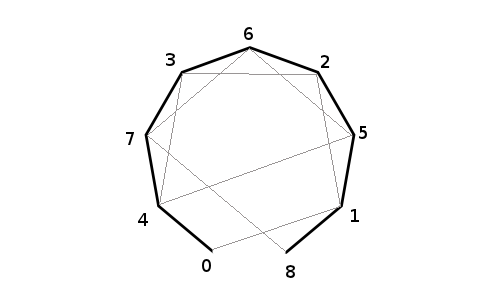
\includegraphics[scale=0.6]{images/rev_grafo_bkp.png} 
  \caption{Grafo de \bkp{} da permutação $\pi = (~4~7~3~6~2~5~1~)$.}
  \label{fig:rev_grafo_bkp}
\end{figure}

Usando o conceito de \bkp{}, temos que uma reversão atua em dois
pontos em uma permutação e, portanto, pode reduzir o número de \bkp{}
em pelo menos um e no máximo dois~\cite{BafnaPevzner*1996}, levando ao
Teorema~\ref{teo:rev_bkp_bound}. 

\begin{teo}
\label{teo:rev_bkp_bound}
Para qualquer permutação $\pi$, 
\[\frac{1}{2} b_r(\pi) \leq d_r(\pi) \leq
  b_r(\pi).
\]
\end{teo}

Um ciclo em $G(\pi)$ é chamado de \textit{alternado} se as cores de
duas arestas consecutivas são diferentes ao longo do ciclo. Assim
dizemos que todos os ciclos pertencentes ao grafo serão ciclos
alternados. O \textit{comprimento} de um ciclo é a sua quantidade de
arestas pretas. Um $k$-ciclo é um ciclo que contem $k$ arestas
negras. Um \textit{ciclo longo} é um ciclo de comprimento maior que
dois.

Observe que $G(\pi)$ pode ser decomposto em ciclos de arestas
disjuntas, pois cada vértice tem o mesmo número de arestas incidentes
cinzas e pretas. Logo existem diversas maneiras de realizar a
decomposição de ciclos em $G(\pi)$. A
Figura~\ref{fig:rev_grafo_bkp_dec2cic} mostra um exemplo de
decomposição em ciclos para o grafo de \bkp{} da permutação $\pi =
(~4~7~3~6~2~5~1~)$.

\begin{figure}[h]
  \centering 
  \begin{tabular}{ccc} 
  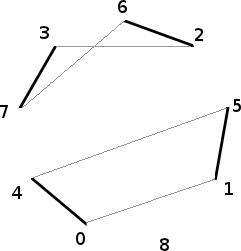
\includegraphics[scale=0.6]{images/rev_grafo_bkp_dec2cic-1.png}
  & ~~~~
  & 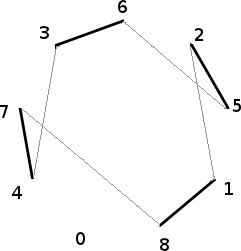
\includegraphics[scale=0.6]{images/rev_grafo_bkp_dec2cic-2.png} 
  \end{tabular} 
  \caption{Exemplo de decomposição em ciclos de arestas disjuntas para
  o grafo de \bkp{} da permutação $\pi = (~4~7~3~6~2~5~1~)$.}
  \label{fig:rev_grafo_bkp_dec2cic}
\end{figure}

Uma reversão atua em duas arestas pretas de $G(\pi)$, se estas arestas
representam os \bkp{} que são separados pela operação de
reversão~\cite{Christie*1998}. O Teorema~\ref{teo:rev_cic_bound},
demonstrado no trabalho de Christie~\cite{Christie*1998}, fornece os
limitantes para a distância de reversão usando a quantidade de
$2$-ciclos na máxima decomposição em ciclos de $G(\pi)$.

\begin{teo}
\label{teo:rev_cic_bound}
Se $c_{2}(\pi)$ é o número mínimo de $2$-ciclos em qualquer máxima
decomposição em ciclos de $G(\pi)$ então: 
\[
\frac{2}{3} b_r(\pi)
- \frac{1}{3} c_{2}(\pi) \leq d_r(\pi) \leq b_r(\pi) - \frac{1}{2}
c_{2}(\pi).
\]
\end{teo}

\section{Ordenação por Transposições}
\label{sec:trans}
% transposicoes
Um evento de transposição ocorre quando dois blocos adjacentes no
genoma trocam de posição. Uma transposição $\rho(i, j, k)$, para
$1 \leq i < j < k \leq n + 1$, aplicada ao genoma $\pi =
(~\pi_{1}~\pi_{2}~\ldots~\pi_{n}~)$ gera a permutação $\rho\pi =
(\pi_{1}~\ldots~\pi_{i-1}~\pi_{j}~\ldots~\pi_{k-1}~\pi_{i}~\ldots$
$\pi_{j-1}~\pi_{k}~\ldots~\pi_{n})$ (Figura~\ref{fig:transposition}).

\begin{figure}[h]
  \centering
  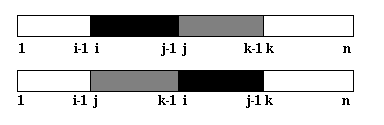
\includegraphics{images/transposition.png} 
  \caption{Transposição aplicada em uma permutação.}
  \label{fig:transposition}
\end{figure}

A distância de transposição $d_{t}(\pi, \sigma)$ entre duas
permutações $\pi$ e $\sigma$ é o número mínimo $t$ de transposições
$\rho_{1}, \rho_{2}, \ldots, \rho_{t}$ tal que
$\pi \rho_{1} \rho_{2} \ldots \rho_{t} = \sigma$. Note que a distância
de transposição entre $\pi$ e $\sigma$ é igual à distância de transposição
entre $\sigma^{-1} \pi$ e $\iota$. Então, sem perda de generalidade,
podemos dizer que o problema da distância de transposição é
equivalente ao problema de ordenação por transposições, que é a
distância de transposição entre a permutação $\pi$ e a permutação
identidade $\iota$, denotado por $d_{t}(\pi)$.

Este problema foi estudado por Bafna e
Pevzner~\cite{BafnaPevzner*1998}, onde apresentaram um algoritmo capaz
de fornecer uma resposta aproximada na razão de $1.5$, além de derivar
um importante limitante inferior para o problema. Introduziram o
conceito de \bkp{} em eventos de transposições, elementos adjacentes
em um genoma, mas não no outro, e o conceito de grafo de ciclos, ambos
ferramentas importantes utilizadas para encontrar limitantes para o
problema. Foram apresentados várias questões em aberto como verificar
a complexidade do problema da distância de transposição e o diâmetro,
que é a maior distância possível entre duas permutações de tamanho
$n$. O problema do diâmetro foi estudado por Meidanis, Walter e
Dias~\cite{MeidanisWalterDias*1997}.

A complexidade deste problema ficou em aberto por um longo tempo. O
trabalho de Bulteau, Fertin e Rusu~\cite{BulteauFertinRusu*2010}
apresentou a prova de que o problema de ordenação por transposição
pertence a classe dos problemas NP-Difíceis. Elias e
Hartman~\cite{EliasHartman*2006} apresentaram um algoritmo de
aproximação na razão de $1.375$. O trabalho de
Labarre~\cite{Labarre*2006} apresentou novos limitantes, além de
definir classes de permutações em que a distância de transposição pode
ser calculada em tempo e espaço lineares.

Nas subseções~\ref{subsec:trans_bkp} e~\ref{subsec:trans_cycle_graph}
apresentam ferramentas usadas para encontrar limitantes para o
problema de ordenação por transposições. Os limitantes usados neste
projeto estão descritos na subseção~\ref{subsec:trans_limitantes}.

\subsection{Breakpoints}
\label{subsec:trans_bkp}
No problema de ordenação por transposições, um \bkp{} é um par
$(\pi_{i}, \pi_{i+1})$ tal que $\pi_{i+1} \neq \pi_{i} + 1$. Denota-se
por $b_{t}(\pi)$ como sendo o número de \bkp{} na permutação $\pi$.

\subsection{Grafo de ciclos}
\label{subsec:trans_cycle_graph}
O conceito de grafo de ciclos foi introduzido por Bafna e
Pevzner~\cite{BafnaPevzner*1998} e foi usado para obter limitantes
melhores para o problema.

Um grafo direcionado com arestas coloridas, denotado por $G(\pi)$, é
chamado de grafo de ciclos da permutação $\pi$ se possui um conjunto
de vértices $\{0,~1,~\ldots~,~n+1\}$ e seu conjunto de arestas é
definido como para todo $1 \leq i \leq n+1$, arestas cinzas são
direcionadas de $i-1$ para $i$ e arestas pretas de $\pi_{i}$ para
$\pi_{i-1}$. A Figura~\ref{fig:trans_cycle_graph} mostra o grafo de
ciclos para a permutação $\pi = (~4~7~3~6~2~5~1~)$.

\begin{figure}[h]
  \centering 
  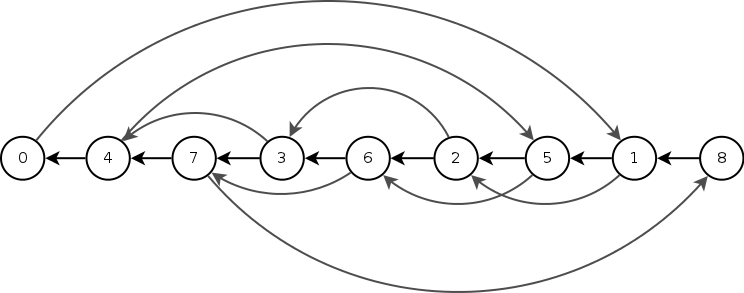
\includegraphics[scale=0.6]{images/trans_cycle_graph.png} 
  \caption{Grafo de ciclos para a permutação $\pi = (~4~7~3~6~2~5~1~)$.}
  \label{fig:trans_cycle_graph}
\end{figure}

\subsection{Limitantes}
\label{subsec:trans_limitantes}
Para o problema de ordenação por transposições usamos três tipos de
limitantes:

\begin{itemize}
\item{\textit{tra\_def}. 
Este é o limitante padrão, com limite inferior igual à $0$ e limite
superior igual a $n$ (tamanho da permutação).}
\item{\textit{tra\_br}.
Usando o conceito de \bkp{} em transposições, sabemos que uma
transposição atua em três pontos de uma permutação, logo, pode reduzir
o número de \bkp{} em pelo menos um e no máximo
três~\cite{BafnaPevzner*1998}, levando ao
Teorema~\ref{teo:trans_br_bound}.

\begin{teo}
  \label{teo:trans_br_bound}
  Para qualquer permutação $\pi$, $\frac{b_t(\pi)}{3} \leq d_t(\pi) \leq
  b_t(\pi)$.
\end{teo}
}
\item{\textit{tra\_cg}.
Usando o conceito de grafo de ciclos, um ciclo alternado de $G(\pi)$ é
ciclo direcionado com arestas de cores alternadas. Para todo vértice
de $G(\pi)$ toda aresta chegando é unicamente pareada com uma aresta
saindo de cor diferente. Isto implica que existe uma decomposição
única de ciclos alternados do conjunto de arestas de $G(\pi)$. A
seguir o termo ciclo é usado no lugar de ciclos alternados e usamos o
termo $k-\text{ciclo}$ para definir um ciclo alternado de tamanho $2k$,
$k-\text{ciclo}$ é longo se $k > 2$, e curto caso contrário.

Para melhorar o limitante, Bafna e Pevzner~\cite{BafnaPevzner*1998}
estudou separadamente os ciclos pares e ímpares. Um ciclo é impar se
número ímpar de arestas pretas e par caso contrário. Seja
$c_{ímpar}(\pi)$ o número de ciclos ímpares de $G(\pi)$, para uma
permutação $\pi$, e $\Delta c_{ímpar} (\rho) = c_{ímpar} (\pi \rho) -
c_{ímpar} (\pi)$ a mudança no número de ciclos ímpares devido a
transposição $\rho$, temos que $\Delta c_{ímpar} \in \{2, 0, -2\}$,
gerando o resultado do Teorema~\ref{teo:trans_cg_bound}.

\begin{teo} 
  \label{teo:trans_cg_bound} 
  Para qualquer permutação $\pi$, $\frac{n + 1 - c_{ímpar}(\pi)}{2} \leq
  d_t(\pi) \leq \frac{3}{4} (n + 1 - c_{ímpar}(\pi))$.
\end{teo}
}
\end{itemize}


\section{Ordenação por Reversões e Transposições}
\label{sec:rev_trans}
% reversoes e transposicoes
Na natureza um genoma não sofre apenas eventos de reversão ou de
transposição, ele está exposto a diversos eventos diferentes. Para
esta situação, iremos estudar o caso onde os eventos de reversão e
transposição ocorrem simultaneamente sobre um genoma.

A distância de reversão e transposição $d_{rt}(\pi, \sigma)$ entre
duas permutações $\pi$ e $\sigma$ é o número mínimo $rt$ de reversões
e transposições $\rho_{1}, \rho_{2}, \ldots, \rho_{rt}$ tal que
$\pi \rho_{1} \rho_{2} \ldots \rho_{rt} = \sigma$. Como no caso em que
os eventos ocorrem individualmente, podemos dizer, sem perda de
generalidade, que o problema da distância de reversão e transposição é
equivalente ao problema de ordenação por reversões e transposições,
que é a distância de reversão e transposição entre a permutação $\pi$ e a
permutação identidade $\iota$, denotado por $d_{rt}(\pi)$.


